% ----------------------------------------------------------------
% Article Class (This is a LaTeX2e document)  ********************
% ----------------------------------------------------------------
\documentclass[article]{IEEEtran}
\usepackage[english]{babel}
\usepackage{amsmath,amsthm}
\usepackage{amsfonts}
\usepackage{array}
\usepackage{multirow}
\usepackage{graphicx}
\usepackage{epstopdf}
\usepackage{color}
\usepackage[tight,footnotesize]{subfigure}
\usepackage{indentfirst}
\usepackage{cite}
\usepackage{mdwmath}
\usepackage{mdwtab}
\usepackage[linesnumbered,ruled]{algorithm2e}
\usepackage{url}
%\usepackage{caption}

% THEOREMS -------------------------------------------------------
\newtheorem{thm}{Theorem}[section]
\newtheorem{cor}[thm]{Corollary}
\newtheorem{lem}[thm]{Lemma}
\newtheorem{prop}[thm]{Proposition}
\theoremstyle{definition}
\newtheorem{defn}[thm]{Definition}
\theoremstyle{remark}
\newtheorem{rem}[thm]{Remark}
\numberwithin{equation}{section}
% ----------------------------------------------------------------
\IEEEoverridecommandlockouts% enable thanks

\begin{document}

\title{Scalable $K$-Order LCP Array Construction for Massive Data}

\author{\IEEEauthorblockN{Yi~Wu$^1$, Junwei Liu$^2$, Ge~Nong$^{3*\thanks{$^*$Corresponding author.}}$, Wai Hong Chan$^4$} \\
\IEEEauthorblockA{$^{1,2,3}$Department of Computer Science and Technology, Sun Yat-sen University, Guangzhou, China \\
$^3$SYSU-CMU Shunde International Joint Research Institute, Shunde, China. \\
$^4$Department of Mathematics and Information Technology, Hong Kong Institute of Education, Hong Kong. \\
Email: $^*$issng@mail.sysu.edu.cn
}}

% ----------------------------------------------------------------
\maketitle

\begin{abstract}
    A new method is proposed to compute the $K$-order longest common prefix (LCP) array for a size-$n$ input string $T$ with its suffix array, where the maximum LCP of a pair of suffixes of $T$ is truncated to be at most $K$ characters. By employing a finger-printing function, string comparisons are translated into integer comparisons that can be accomplished in constant time. This method can be applied on the internal memory and easily extended to both external memory and distributed computation models. For each of these models, the total time and space complexities are $\mathcal{O}(n\log K)$ and $\mathcal{O}(n)$, respectively. In particular, this method is scalable for a distributed model of $d$ computing nodes, where the time and space complexities are evenly divided onto each node as $\mathcal{O}((n\log K)/d)$ and $\mathcal{O}(n/d)$, respectively.
\end{abstract}

\begin{IEEEkeywords}
$K$-order LCP array, suffix array, finger-printing, external and distributed models.
\end{IEEEkeywords}


% ----------------------------------------------------------------
\section{Introduction}
Suffix array~(SA)~\cite{Manber1993} is a succinct data structure for full-text indexing. In conjunction with the longest common prefix array~(LCPA), SA can emulate a bottom-up or top-down traversal of the corresponding suffix tree and thus becomes popular for a variety of string processing tasks previously tackled by suffix tree~\cite{Abouelhodaa2004}.

As far as we know, the most time and space efficient SA and LCPA construction algorithms designed for random access memory~(RAM) model are based on the induced sorting principle~\cite{nong2011,Fischer11}. However, great improvements in data sampling techniques have created new challenges as the ever-increasing data sets can no longer be processed internally. To close the gap, recently, three novel algorithms~\cite{Nong15, Bingmann12, Nong14} have been designed to adapt the internal SA construction algorithm SA-IS~\cite{nong2011} for sorting suffixes in external memory and achieved remarkable performance gains against the previous state-of-the-art~\cite{Dementiev08}. In particular, the eSAIS algorithm~\cite{Bingmann12} can also produce the LCPA together with the construction of suffix array, where the overhead of time and I/O volume is twice as that of the plain SA construction. The eGSA algorithm~\cite{Felipe2013} enables the simultaneous computation of SA and LCPA for data sets composed of multiple strings of variable-lengths by using multi-way merge-sort, where the time spent in construction is reduced to one-third of eSAIS. The exLCP algorithm~\cite{Markus2012} is a lightweight LCPA construction algorithm for very large collections of sequences, where the Burrow-Wheeler transform is calculated at the same time to facilitate the computation. Given the suffix array as input, the LCPscan algorithm \cite{Juha2014} builds the LCPA from the permuted LCPA and inverse SA computed in advance. Compared with eSAIS, LCPscan requires less disk space and performs better in terms of the running time and I/O efficiency. While these algorithms achieve remarkable time and space performance, however, their designs are quite sophisticated and not trivial to be extended for parallel and distributed models so as to scale the performance by a cluster of computers, for example.

It has been observed from~\cite{Felipe2013} that the average LCPs are typically small for realistic data, especially in genome data sets such as protein and DNA. This motivated us to design a practical algorithm for computing the $K$-order LCPA of input string $T$, where the maximum LCP of any two suffixes in $T$ is assumed to be no more than $K<<|T|$~(e.g. $K=8192$).

The contributions of this work are mainly two aspects:
\begin{enumerate}
\item Our first contribution is to design and implement a $K$-order LCPA construction method applicable to typical internal and external memory models, which can build the LCPA in $\mathcal{O}(n\log K)$ time and $\mathcal{O}(n)$ space using the LCP batch querying technique~(LCP-BQT)~\cite{Philip2013} previously proposed for sparse SA construction. This method can be easily applied on both the internal and the external models. The program that we developed for the external memory model is composed of less than 600 code lines in C++.
\item The existing parallel construction algorithms are mainly designed for shared memory models such as bulk synchronous parallel and parallel random access machine~\cite{Shun2014,Deo2013}. Our second contribution is to parallelize the method in a distributed system consisting of $d$ computing nodes.
\end{enumerate}

The rest of the paper is organized as below.
Section~\ref{sec:construction_in_ram} introduces LCP-BQT and describes the algorithmic framework of the proposed method in the RAM model.
Section~\ref{sec:construction_in_em} and~\ref{sec:construction_in_distributed} extend the method to the external memory and distributed models, respectively.
Finally, we give the performance evaluation in Section~\ref{sec:experimental_results} and the conclusion in Section~\ref{sec:conclusion}.

\section{$K$-Order LCPA Construction in RAM}\label{sec:construction_in_ram}

\subsection{Notation}\label{subsec:basic_notations}

Consider an input text $T[0,n-1] =T[0]T[1]...T[n-1]$ of $n$ characters from an ordered alphabet $\Sigma$. We assume $T[n-1]$ to be a unique character alphabetically smaller than any characters in $T[0,n-2]$ and introduce the following notations for description clarity.

\begin{itemize}
\item ${\sf pre}(T,i)$ and ${\sf suf}(T,i)$: We write ${\sf pre}(T,i)$ to be the prefix of $T$ running from $T[0]$ to $T[i]$ and write ${\sf suf}(T,i)$ to be the suffix of $T$ running from $T[i]$ to $T[n-1]$.
\item  $SA_T$:  The suffix array of $T$, denoted by $SA_T$, is a permutation of integers $[0,n)$ such that ${\sf suf}(T,SA_T[0])<{\sf suf}(T,SA_T[1])<...<{\sf suf}(T,SA_T[n-1])$ in their lexicographic order.
\item ${\sf lcp}(i,j)$ and $LCPA_T$: We write ${\sf lcp}(i,j)$ to be the LCP length of ${\sf suf}(T,i)$ and ${\sf suf}(T,j)$. The LCPA of $T$, denoted by $LCPA_T$, consists of $n$ integers taken from $[0,n)$, where $LCPA_T[i]= {\sf lcp}(SA_T[i],SA_T[i-1])$.
\item $\Delta_{k}$: We denote $2^{\log n - k - 1}$ by $\Delta_{k}$.
\end{itemize}

\subsection{LCP Batch Querying Technique}\label{subsec:lcp_batch_querying_technique}

Given $T$ and a set of $b$ pairs of indices $P$, LCP-BQT computes ${\sf lcp}(i,j)$ for all pairs $(i,j)\in P$ in $\mathcal{O}(n\log b)$ time using $\mathcal{O}(n)$ RAM space. The main idea behind the technique is to find the indices $(i_{fin}, j_{fin})$ for $(i,j)$ such that $T[i,i_{fin}-1]=T[j,j_{fin}-1]$ and $T[i_{fin}] \neq T[j_{fin}]$. To do this, it initially assigns $P$ to $P_0$ and performs a loop of $\log b$ rounds on the set, where the goal of round $k\in [0,\log b)$ is to decide whether ${\sf lcp}(i_k,j_k) \le \Delta_k$ or not for each pair $(i_k,j_k)\in P_k$ and generate $P_{k+1}$ as the input for round $k+1$ as following: if $T[i_k,i_k+\Delta_k-1] \neq T[j_k,j_k+\Delta_k-1]$, then insert $(i_k,j_k)$ into $P_{k+1}$; otherwise, insert $(i_k+\Delta_k,j_k+\Delta_k)$ into $P_{k+1}$. The string comparison in concern can be carried out by scanning the two strings from left to right and literally comparing the characters in their lexicographic order. However, this operation takes $O(2^{\log n})$ time at worst and thus becomes a performance bottleneck.

As a solution to relieving the time overhead, the finger-printing function presented in~\cite{Karp1987} is introduced herein for transforming string comparisons to their integer counterparts that can be done in constant time. The finger-print~(FP) of $T[i,j]$, namely $FP[i,j]$, is calculated by the formula $FP[i,j] = \sum_{p=i}^{j} \delta^{j-p} \cdot T[p] \, mod \, L$, in which $L$ is a prime and $\delta$ is an integer randomly chosen from domain $[1,L)$. Obviously, two identical strings always have a common finger-print, while the converse is not true. Fortunately, it has been proved that the error probability of two different strings having a same finger-print can be ignored when $L$ is very large.

Following the above description, the 3-step algorithmic framework for round $k$ is given below.

\begin{enumerate}
\item Scan $T$ rightward to iteratively compute the finger-print of ${\sf pre}(0,l)$ by the formula $FP[0,l] = FP[0,l-1] \cdot \delta + T[l] \,\, mod \,\, L$ and store $FP[0,l]$ in the hash table if $l\in \{ \{i_k-1\}\cup\{j_k-1\}\cup\{i_k +\Delta_{k} - 1\}\cup\{j_k+ \Delta_{k} - 1\},(i_k,j_k)\in P_k\}$.
\item For each $l\in \{\{i_k\}\cup \{j_k\}$, $(i_k,j_k)\in P_k\}$, compute the finger-print of $T[l,l+\Delta_{k} - 1]$ by the formula $FP[l,l+ \Delta_{k} - 1]=FP[0,l+ \Delta_{k} - 1] - FP[0,l-1] \cdot \delta^{\Delta_{k}} \, mod \, L$, where $FP[0,l+ \Delta_{k} - 1]$ and $FP[0,l-1]$ can be retrieved from the hash table in amortized $\mathcal{O}(1)$ time.
\item For each pair $(i_k,j_k)\in P_k$, compare $FP[i_k,i_k+\Delta_{k} - 1]$ with $FP[j_k,j_k+\Delta_{k} - 1]$. If equal, insert $(i_k+\Delta_{k},j_k+\Delta_{k})$ into $P_{k+1}$; otherwise, insert $(i_k, j_k)$ into $P_{k+1}$.
\end{enumerate}

The following two properties remain invariant during the whole loop.

\begin{itemize}
\item At the beginning of round $k$, ${\sf lcp}(i_k,j_k) \le 2 \cdot \Delta_{k}$ for each pair $(i_k,j_k) \in P_k$.
\item At the end of round $k$, ${\sf lcp}(i_{k+1},j_{k+1}) \le \Delta_{k}$ for each pair $(i_{k+1},j_{k+1}) \in P_{k+1}$.
\end{itemize}

After the loop, we have ${\sf lcp}(i_{\log b},j_{\log b}) \le \frac{n}{b}$ for each pair $(i_{\log b},j_{\log b}) \in P_{\log b}$, and thus can compute ${\sf lcp}(i_{\log b}, j_{\log b})$ in $\mathcal{O}(\frac{n}{b})$ time by literally compare the characters in ${\sf suf}(T,i_{\log b})$ and ${\sf suf}(T,j_{\log b})$ from left to right. Let $i_{fin} = i_{\log b} + {\sf lcp}(i_{\log b}, j_{\log b})$ and $j_{fin}= j_{\log b} + {\sf lcp}(i_{\log b}, j_{\log b})$, then $i_{fin}$ and $j_{fin}$ are the position indices to the right side of $i$ and $j$ such that $T[i,i_{fin}-1] = T[j,j_{fin}-1]$ and $T[i_{fin}] \neq T[j_{fin}]$.

\begin{lem}
\label{thm:lcp:naive}
The LCP of any $b$ pairs of suffixes in $T$ can be correctly computed in $\mathcal{O}(n\log b)$ time using $\mathcal{O}(b)$ RAM space with a high probability.
\end{lem}
Proof. The time complexity of LCP-BQT is dominated by the loop of $\log b$ rounds, where each round takes $\mathcal{O}(n)$ time for step 1 to iteratively compute the finger-prints of ${\sf pre}(T,l)$, and $\mathcal{O}(b)$ time for steps 2-3 to compute and compare the finger-prints of strings. The space in need is limited to $\mathcal{O}(b)$ words by employing a hash table for storing and retrieving the finger-prints.


\subsection{Details}\label{subsec:implementation_in_ram}

We exploit the use of LCP-BQT by converting the K-order LCPA construction problem to the computation of ${\sf lcp}(i,j)$ for all pairs of position indices in $\{(SA_T[1], SA_T[0]),(SA_T[2], SA_T[1])\ldots (SA_T[n], SA_T[n-1])\}$. For presentation clarity, parameters and notations listed below are introduced to the design of internal memory algorithm lcpa-ram, where $i\in [0,n)$ and $k\in [0,\log K)$.

\begin{itemize}
\item $CP_k$ and $PP_k$: integer arrays of size $2n$, in which the two substrings $T[CP_k[2i],CP_k[2i+1]]$ and $T[PP_k[2i],PP_k[2i+1]]$ are compared to determine their LCP.
\item $ICP_k$ and $IPP_k$: integer arrays of size $2n$, which are produced by radix-sorting $CP_k$ and $PP_k$, respectively.
\item $HT$: a hash table for storing and retrieving finger-prints of ${\sf pre}(T,i)$, where $i\in \{CP_k[j] \cup PP_k[j], j\in[0,2n)\}$.
\end{itemize}




\begin{algorithm}[hbtp!]
\caption{Compute $K$-Order $LCPA_T$ in RAM}
\label{fig:alg:ram}
lcpa-ram($T$, $SA_T$, {\em n}, $K$, $HT$){\\
\SetAlgoNoLine
Scan $SA_T$ rightward to produce $CP_0$ and $PP_0$. \\
Let $k = 0$. \\
\While{$k < \log K$}{
\Indentp{-1em}
Radix-sort $CP_k$ and $PP_k$ to produce $ICP_k$ and $IPP_k$. \\
For $i\in [0,n)$, scan $T$ rightward to compute the finger-print of ${\sf pre}(T,i)$ and let $FP[0,i]=HT[i]$ if $i\in \{ICP_k[j] \cup IPP_k[j], j\in[0,2n)\}$. \\
For $i\in [0,n)$, scan $CP_k$ and $PP_k$ rightward to compute and compare $FP[CP_k[2i]+1,CP_k[2i+1]]$ and $FP[PP_k[2i]+1,PP_k[2i+1]]$ for generating $CP_{k+1}$ and $PP_{k+1}$. \\
Let $k = k +1$ and clear $HT$. \\
}
For $i\in [0,n)$, scan $T$, $CP_{\log K}$ and $PP_{\log K}$ rightward to compute $\Upsilon_i = {\sf lcp}(CP_{\log K}[2i],PP_{\log K}[2i])$. \\
For $i\in [0,n)$, let ${\sf lcp}(SA_T[i],SA_T[i-1])=CP_{\log K}[2i] +\Upsilon_i-SA_T[i]$. \\
}
\end{algorithm}



At the very beginning, Algorithm~\ref{fig:alg:ram} computes $CP_0$ and $PP_0$ as following: 1) $CP_0[2i]=SA_T[i]-1$ and $CP_0[2i+1]=SA_T[i]+ \Delta_0 - 1$; and 2) $PP_0[2i]=SA_T[i-1]-1$ and $PP_0[2i+1]=SA_T[i-1]+ \Delta_0 - 1$. When finishing the computation, it proceeds on to performing a loop of $\log K$ rounds in lines 4-9. A key operation in round $k$ is to radix-sorts entries in $CP_k$ and $PP_k$ for iteratively computing the finger-prints of ${\sf pre}(T,l)$. Afterward, these values are retrieved from the hash table to compute and compare the finger-prints of $T[CP_k[2i]+1,CP_k[2i+1]]$ and $T  [PP_k[2i]+1,PP_k[2i+1]]$ for producing $CP_{k+1}$ and $PP_{k+1}$. More specifically, increase $CP_{k}[2i]$ and $PP_{k}[2i]$ by $\Delta_k$ and $CP_{k}[2i+1]$ and $PP_{k}[2i+1]$ by $\Delta_{k+1}$ if the two finger-prints are identical; otherwise, decrease $CP_{k}[2i+1]$ and $PP_{k}[2i+1]$  by $\Delta_{k+1}$. The algorithm then assigns $CP_k$ and $PP_k$ to $CP_{k+1}$ and $PP_{k+1}$, respectively. After the while-loop, it takes $\mathcal{O}(n)$ time to compute the LCP array in lines 10-11 as ${\sf lcp}(CP_{\log K}[2i],PP_{\log K}[2i]) \le 1$ holds for any $i \in [0,n)$. This leads us to the conclusion stated below.

\begin{lem}
\label{thm:lcp:ram}
Given $T$ and $SA_T$, the $K$-order $LCPA_T$ can be correctly computed in $\mathcal{O}(n\log K)$ time using $\mathcal{O}(n)$ RAM space with a high probability.
\end{lem}
Proof. With respect to time complexity, the while-loop spends $\mathcal{O}(n\log K)$ time computing $CP_{\log K}$ and $PP_{\log K}$. On the other respect, it demands $\mathcal{O}(n)$ internal space to maintain $HT$, $CP_k$ and $PP_k$.

\section{$K$-Order LCPA Construction in Disk}\label{sec:construction_in_em}

A hash table is employed in Algorithm~\ref{fig:alg:ram} to store the finger-prints for quick lookups. This is feasible in the RAM model, but not practical when {\em n} becomes larger as the table can not be wholly afforded internally anymore. For the purpose, we reformulate lcpa-ram to design a disk-friendly external memory algorithm, called lcpa-disk, where the finger-prints in use are sequentially retrieved from the external memory.

\subsection{Notation}

Given the RAM capacity $M$ in our external memory model, $T$ and $SA_T$ are evenly partitioned into $d=n/m$ blocks, where each block is of size $m=O(M)$ and thus can be processed as a whole in RAM. We extend $CP_k$ and $PP_k$ previously exploited in lcpa-ram to define their counterparts $ECP_k$ and $EPP_k$. Both of them consist of $2n$ entries and each entry is a tuple of $\langle idx, pos, fp \rangle$ as described below.
\begin{itemize}
\item $idx$: the index of the entry in $ECP_k/EPP_k$, where $ECP[i].idx=EPP[i].idx=i$.
\item $pos$: the ending position index of ${\sf pre}(0,pos)$ in $T$.
\item $fp$: the finger-print of ${\sf pre}(0,pos)$.
\end{itemize}

For $i\in [0,n)$, the $fp$ values of $ECP_k[2i]$ and $ECP_k[2i+1]$ are employed to figure out $FP[ECP_k[2i].pos+1, ECP_k[2i+1].pos]$ by the formula $ECP_k[2i+1].fp - ECP_k[2i].fp \cdot \delta^{\Delta_k} \, mod \, L$, where $FP[EPP_k[2i].pos+1, EPP_k[2i+1].pos]$ can be obtained in a similar way.

\subsection{Details}
Differentiate from Algorithm~\ref{fig:alg:ram}, lcpa-disk performs two runs of external memory sort to arrange fixed-size entries by their integer keys of $\log n$ bits during each round. Specifically, entries in $ECP_k$ and $EPP_k$ are sorted by $pos$ to form $IECP_k$ and $IEPP_k$ in line 5, and sorted back by $idx$ to their original order in line 7. The first sort is for iteratively computing the finger-print of ${\sf pre}(0,pos)$. During the process, we record the computation result in the $fp$ field of each entry instead of a hash table. After the second sort, these values are used to produce $ECP_{k+1}$ and $EPP_{k+1}$ following the same way adopted in lcpa-ram. Given $M=\Omega(nW)^{0.5}$, where $W$ is the size of {I/O} buffers large enough to amortize the overhead of accesses to disks, each run can be done in $\mathcal{O}(n)$ time and space by adopting a multi-way external memory radix-sort of two passes, of which the first pass sorts the lowest $0.5\log n$ bits and the second pass sorts the highest $0.5\log n$ bits. Thus we can come to the following statement.

\begin{lem}
\label{thm:lcp:em}
Given $T$ and $SA_T$, the $K$-order $LCPA_T$ can be correctly computed in $O(n \log K)$ time using $O(n)$ disk space with a high probability.
\end{lem}

\begin{algorithm}[hbtp!]
\caption{Compute $K$-Order $LCPA_T$ in Disk}
\label{fig:alg:em}
lcpa-disk($T$, $SA_T$, {\em n}, $K$){\\
\SetAlgoNoLine
Scan $SA_T$ rightward to produce $ECP_0$ and $EPP_0$.\\
Let $k = 0$. \\
\While{$k < \log K$}{
\Indentp{-1em}
Radix-sort $ECP_k$ and $EPP_k$ by $pos$ to produce $IECP_k$ and $IEPP_k$. \\
For $i\in [0,n)$ and $j\in [0,2n)$, scan $T$ rightward to iteratively compute the finger-print of ${\sf pre}(T,i)$ and assign $FP[0,i]$ to $IECP_k[j].fp$ or $IEPP_k[j].fp$ if $IECP_k[j].pos = i$ or $IEPP_k[j].pos = i$. \\
Radix-sort $IECP_k$ and $IEPP_k$ by $idx$ to reproduce $ECP_k$ and $EPP_k$. \\
For $i \in [0,n)$, scan $ECP_k$ and $EPP_k$ rightward to compute and compare each pair of $(FP[ECP_k[2i].pos+1,ECP_k[2i+1].pos], FP[EPP_k[2i].pos+1,EPP_k[2i+1].pos])$ for generating $ECP_{k+1}$ and $EPP_{k+1}$. \\
Let $k = k + 1$. \\
}
For $i \in [0,n)$, scan $T$, $ECP_{\log K}$ and $EPP_{\log K}$ rightward to compute $\Upsilon_i = {\sf lcp}(ECP_{\log K}[2i].pos,EPP_{\log K}[2i].pos)$. \\
For $i \in [0,n)$, let ${\sf lcp}(SA_T[i],SA_T[i-1])=ECP_{\log K}[2i].pos+\Upsilon_i-SA_T[i]$.\\
}
\end{algorithm}

\subsection{Optimization}\label{subsec:optimization}

The $logK$-round while-loop is time-consuming in lcpa-disk. The algorithm can be adapted to generate $ECP_{k+2}\backslash EPP_{k+2}$ directly from $ECP_k\backslash EPP_k$ so that the number of loop rounds can be reduced by half. To this end, the procedure in lines 8-9 is reformulated as below.

\begin{enumerate}
\item Compute and compare the finger prints of $T[ECP_k[2i].pos+1,ECP_k[2i+1].pos]$ and $T[EPP_k[2i].pos+1,EPP_k[2i+1].pos]$. If equal, perform S2; otherwise, go to S3.
\item Compute and compare the finger-prints of $T[ECP_k[2i+1].pos+1,ECP_k[2i+1].pos+\Delta_{k+1}]$ and $T[EPP_k[2i+1].pos+1,EPP_k[2i+1].pos+\Delta_{k+1}]$. If equal, increase $ECP_k[2i].pos$ and $EPP_k[2i].pos$ by $\Delta_{k}+\Delta_{k+1}$ and $ECP_k[2i+1].pos$ and $EPP_k[2i+1].pos$ by $\Delta_{k+1}+\Delta_{k+2}$; otherwise, increase $ECP_k[2i].pos$ and $EPP_k[2i].pos$ by $\Delta_{k}$ and $ECP_k[2i+1].pos$ and $EPP_k[2i+1].pos$ by $\Delta_{k+2}$.
\item Compute and compare the finger-prints of $T[ECP_k[2i].pos+1,ECP_k[2i].pos+\Delta_{k+1}]$ and $T[EPP_k[2i].pos+1,EPP_k[2i].pos+\Delta_{k+1}]$. If equal, increase $ECP_k[2i].pos$ and $EPP_k[2i].pos$ by $\Delta_{k+1}$ and decrease $ECP_k[2i+1].pos$ and $EPP_k[2i+1].pos$ by $\Delta_{k+2}$; otherwise, decrease $ECP_k[2i+1].pos$ and $EPP_k[2i+1].pos$ by $\Delta_{k+1}+\Delta_{k+2}$.
\item Let $ECP_{k+2}=ECP_{k}$ and $EPP_{k+2}=EPP_{k}$.
\item Let $k = k+2$.
\end{enumerate}

This method, however, brings about a side effect that the workspace grows nearly twice as the prototype because each entry of $ECP/EPP$ is extended to hold two more finger-prints required for executing step 2 or 3. As with lcpa-disk, the finger-prints in use can be computed in $\mathcal{O}(1)$ time after the rightward scan of $T$ for computing and recording the finger-prints of corresponding prefix substrings. This method can be generalized to merge a number of successive loop rounds into one.  We will show in Section~\ref{sec:experimental_results} that the revised algorithm, namely lcpa-disk-m, can achieve a substantial improvement against lcpa-disk in terms of speed.

\section{$K$-Order LCPA Construction in Distributed System}\label{sec:construction_in_distributed}

In what follows, we demonstrate how to parallelize our external memory algorithms in a distributed system consisting of $d$ computing nodes $\{N_0, N_1, ...N_{d-1}\}$. All nodes are interconnected with each other by a gigabit-switch operating in the full duplex mode where the internal and external memory capacities of each node are $M$ and $E~(>> M)$, respectively.

\subsection{Notation}

For $i\in [0,d)$ and $j\in [0,e)$, we evenly partition $T$ and $SA_T$ into $d=n/e$ blocks of size $e=\mathcal{O}(E)$ and allocate them among the computing nodes in a manner of one block per node as below. Similarly, entries in $ECP_k/EPP_k$ and $IECP_k/IEPP_k$ are also divided and distributed to all the computing nodes. Recall that the external memory algorithms lcpa-disk and lcpa-disk-m compute $ECP_{\log K}$ and $EPP_{\log K}$ via two runs of radix-sort externally. To emulate the procedure in our distributed system illustrated in Fig.~\ref{fig:distributed_system}, we set up a group of sending/receiding buffers in each computing nodes for data transmission during the sorts. The following parameters and notations are introduced for description convenience, where $i,j\in [0,d)$ and $k\in [0,logK)$.

\begin{itemize}
\item $T_i$: the $i$-th block of $T$ on node $N_i$, where $T_i[j] = T[ie+j]$.
\item $SA_{T_i}$: the $i$-th block of $SA_T$ on node $N_i$, where $SA_{T_i}[j] = SA_T[ie+j]$.
\item $ECP_{i,k}/EPP_{i,k}$: the $i$-th block of $ECP_{i,k}/EPP_{i,k}$ on node $N_i$, where $ECP_{i,k}[j] = ECP_k[ie+j]$ and $EPP_{i,k}[j] =  EPP_k[ie+j]$.
\item $IECP_{i,k}/IEPP_{i,k}$: the $i$-th block of $IECP_{i,k}/IEPP_{i,k}$ on node $N_i$, where $IECP_{i,k}[j] = IECP_k[ie+j]$ and $IEPP_{i,k}[j] = IEPP_k[ie+j]$.
\item $SB1_{i,j}$ and $SB2_{i,j}$: create two sending buffers $SB1_{i,j}$ and $SB2_{i,j}$ on node $i$ for every other node $j\ne i$, where $SB1_{i,j}$ and $SB2_{i,j}$ cache the entries of $ECP_{i,k}/IECP_{i,k}$ and $EPP_{i,k}/IEPP_{i,k}$ delivered to node $j$, respectively.
\item $RB1_{i,j}$ and $RB2_{i,j}$: create two receiving buffers $RB1_{i,j}$ and $RB2_{i,j}$ on node $i$ for every other node $j\ne i$, where $RB1_{i,j}$ and $RB2_{i,j}$ cache the entries of $ECP_{j,k}/IECP_{j,k}$ and $EPP_{j,k}/IEPP_{j,k}$ received from node $j$, respectively.
\end{itemize}

\begin{figure}[hbtp]
  \centering
  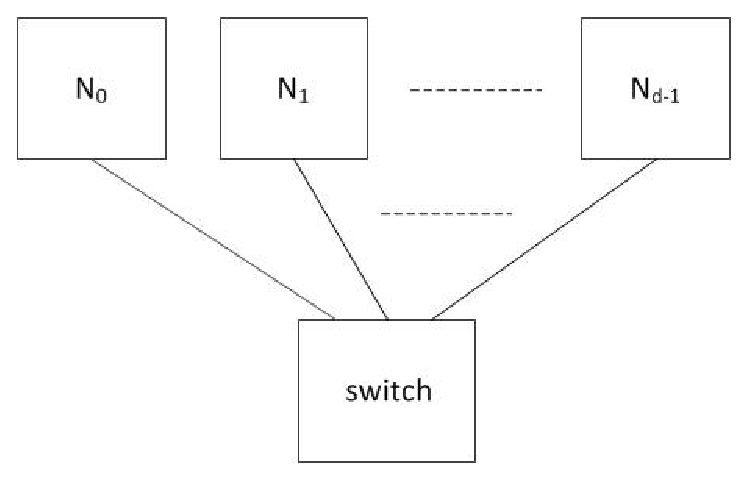
\includegraphics[scale=0.5]{distributed_system.eps}\\
  \caption{Distributed System.}\label{fig:distributed_system}
\end{figure}


\subsection{Detail}

As with lcpa-disk, the distributed algorithm lcpa-ds performs two runs of radix-sorts to compute the $fp$ field of entries in $ECP_k$ and $EPP_k$ by using the sending and receiving buffers. In details, $N_i$ dispatches each entry $x$ in $ECP_{i,k}$ to the sending buffer $SB1_{i,j}$ satisfying $j = x.pos / e$ and delivers them to $N_j$. Upon the arrival of entries from other nodes, $N_j$ radix-sorts entries in $RB1$ by their $pos$ to form $IECP_{j,k}$. Then it scans $T$ from left to right to iteratively compute the finger-prints of required prefix substrings and record them in the $fp$ field of corresponding entries in $IECP_{j,k}$. After that, each entry $y$ in $IECP_{j,k}$ are cached in the sending buffer $SB1_{j,i}$ satisfying $i = y.pos /e$ and forwarded to $N_i$. $N_i$ radix-sorts the received entries in $RB1$ by their $idx$ to regenerate $ECP_{i,k}$. $N_i$ processes entries in $EPP_{i,k}$ following the same way with the help of $SB2_{i,j}$ and $RB2$. $ECP_{i,k+1}$ and $EPP_{i,k+1}$ can be computed by scanning $ECP_{i,k}$ and $EPP_{i,k}$ once. After the while-loop, the LCP array of $T[ie,ie+e)$ can be figured out in linear time according to $ECP_{i,{\log K}}$, $EPP_{i,{\log K}}$ and $SA_{T_i}$ residing on $N_i$. And we can simply concatenate the local LCP array on each node to form $LCP_T$.

\begin{algorithm}[hbtp!]
\caption{Compute $K$-Order $LCPA_T[ie,ie+e)$ on $N_i$}
\label{fig:alg:ds}
lcpa-ds($T_i$, $SA_{T_i}$, $e$, $K$){\\
\SetAlgoNoLine
Scan $T_i$ rightward to compute $ECP_{i,0}$ and $EPP_{i,0}$. \\
Let $k=0$. \\
For $j\in[0,d)$, create sending buffers $SB1_{i,j}$ and $SB2_{i,j}$. \\
Create receiving buffers $RB1_i$ and $RB2_i$. \\
\While{$k < \log K$}{
\Indentp{-1em}
Scan $SA_{T_i}$ rightward to compute $ECP_{i,k}$ and $EPP_{i,k}$. \\
For $j\in[0,d)$ and $p\in[0,2e)$, scan $ECP_{i,k}$ and $EPP_{i,k}$ rightward to cache $ECP_{i,k}[p]$ in $SB1_{i,j}$ or $EPP_{i,k}[p]$ in $SB2_{i,j}$ if $ECP_{i,k}[p].pos$ or $EPP_{i,k}[p].pos$ belongs to $[je,je+e)$. \\
For $j\in[0,d)$, send entries in $SB1_{i,j}$ and $SB2_{i,j}$ to $N_j$. \\
For $j\in[0,d)$, cache entries from $SB1_{i,j}$ and $SB2_{i,j}$ in $RB1_i$ and $RB2_i$. \\
Radix-sort entries in $RB1_i$ and $RB2_i$ by $pos$ to produce $IECP_{i,k}$ and $IEPP_{i,k}$. \\
For $p\in[0,e)$ and $q\in [0,2e)$, scan $T_i$ rightward to iteratively compute the finger-print of ${\sf pre}(T,ie+p)$ and assign $FP[0,ie+p]$ to $IECP_{i,k}[q].fp$ or $IEPP_{i,k}[q].fp$ if $IECP_{i,k}[q].pos = ie+p$ or $IEPP_{i,k}[q].pos = ie+p$. \\
For $j\in[0,d)$ and $p\in[0,2e)$, scan $IECP_i$ and $IEPP_i$ rightward to cache $IECP_{i,k}[p]$ in $SB1_{i,j}$ or $IEPP_{i,k}[p]$ in $SB2_{i,j}$ if $IECP_{i,k}[p].pos$ or $IEPP_{i,k}[p].pos$ belongs to $[je,je+e)$. \\
For $j\in[0,d)$, send entries in $SB1_{i,j}$ and $SB2_{i,j}$ to $N_j$. \\
For $j\in[0,d)$, cache entries from $SB1_{i,j}$ and $SB2_{i,j}$ in $RB1_i$ and $RB2_i$. \\
Radix-sort entries in $RB1_i$ and $RB2_i$ by $idx$ to reproduce $ECP_{i,k}$ and $EPP_{i,k}$. \\
For $p\in [0,e)$, scan $ECP_{i,k}$ and $EPP_{i,k}$ rightward to compute and compare the finger-prints of $T[ECP_{i,k}[2p].pos+1, ECP_{i,k}[2p+1].pos]$ and $T[EPP_{i,k}[2p].pos+1, EPP_{i,k}[2p+1].pos]$ for generating $ECP_{i,k+1}$ and $EPP_{i,k+1}$. \\
Let $k=k+1$. \\
}
For $p\in [0,e)$, scan $T_i$, $ECP_{i,\log K}$ and $EPP_{i,\log K}$ rightward to literally compute $\Upsilon_{i,p}={\sf lcp}(ECP_{i,\log K}[2p].pos,EPP_{i,\log K}[2p].pos)$. \\
For $p\in [0,e)$, let ${\sf lcp}(SA_{T_i}[p],SA_{T,i}[p-1])=ECP_{i,\log K}.pos + \Upsilon_{i,p} - SA_{T_i}[p]$. \\
}
\end{algorithm}

Note that, the internal memory is partitioned into two parts, where the first part is employed to maintain the sending/receiving buffers and the other part is used to establish I/O buffers for reading/writing entries of $ECP_{i,k}$ and $EPP_{i,k}$. High performance can be achieved if the memory capacity spared for these buffers is large enough to compensate the delay of data transmissions and amortize the overhead of I/O operations. Besides, the optimization adopted in lcpa-disk-m can also be used herein to accelerate the speed.

\begin{lem}
\label{thm:lcp:pdm}
Given $T$ and $SA_T$, the $K$-order $LCPA_T$ can be correctly computed in $\mathcal{O}(\frac{n}{d}\log K)$ time using $\mathcal{O}(\frac{n}{d})$ disk space on each computing node with a high probability.
\end{lem}
Proof. Algorithm~\ref{fig:alg:ds} performs radix-sorts among the computing nodes, where the overhead of time and space for data transmission sums up to $\mathcal{O}(e\log K)$ during the whole loop. This is because each node sends and receives $\mathcal{O}(e)$ entries per round.



\section{Experimental Results}\label{sec:experimental_results}

A series of experiments are conducted on a real data set collected from the web site \url{http://download.wikimedia.org/enwiki/} to evaluate the performance of {C++} programs for the external and distributed algorithms presented in Section~\ref{sec:construction_in_em} and~\ref{sec:construction_in_distributed}. The experimental platform for lcpa-disk and lcpa-disk-m is deployed on a computer equipped with 2 Intel Xeron E3-1220 CPUs, 4GiB RAM and a disk of 2TB capacity, while the one for lcpa-ds is set up in a distributed system consisting of four identical computers interconnected with a gigabit switch. Programs are compiled by gcc 4.8.4, running on Ubuntu 14.04 operating system.

Instead of to develop a radix sorter specific for our purpose, we use STXXL~\cite{Dementiev2007} to perform the external memory sorts in our programs. STXXL is a {C++} STL library designed for efficient computation in external memory, and freely available at \url{http://stxxl.sourceforge.net/}. Benefit from the powerful priority queues provided by STXXL, the codes for lcpa-disk, lcpa-disk-m and lcpa-ds are no more than 400, 600 and 700 lines, respectively.

\subsection{lcpa-disk vs. lcpa-disk-m}
\begin{figure}[hbtp]
  \centering
  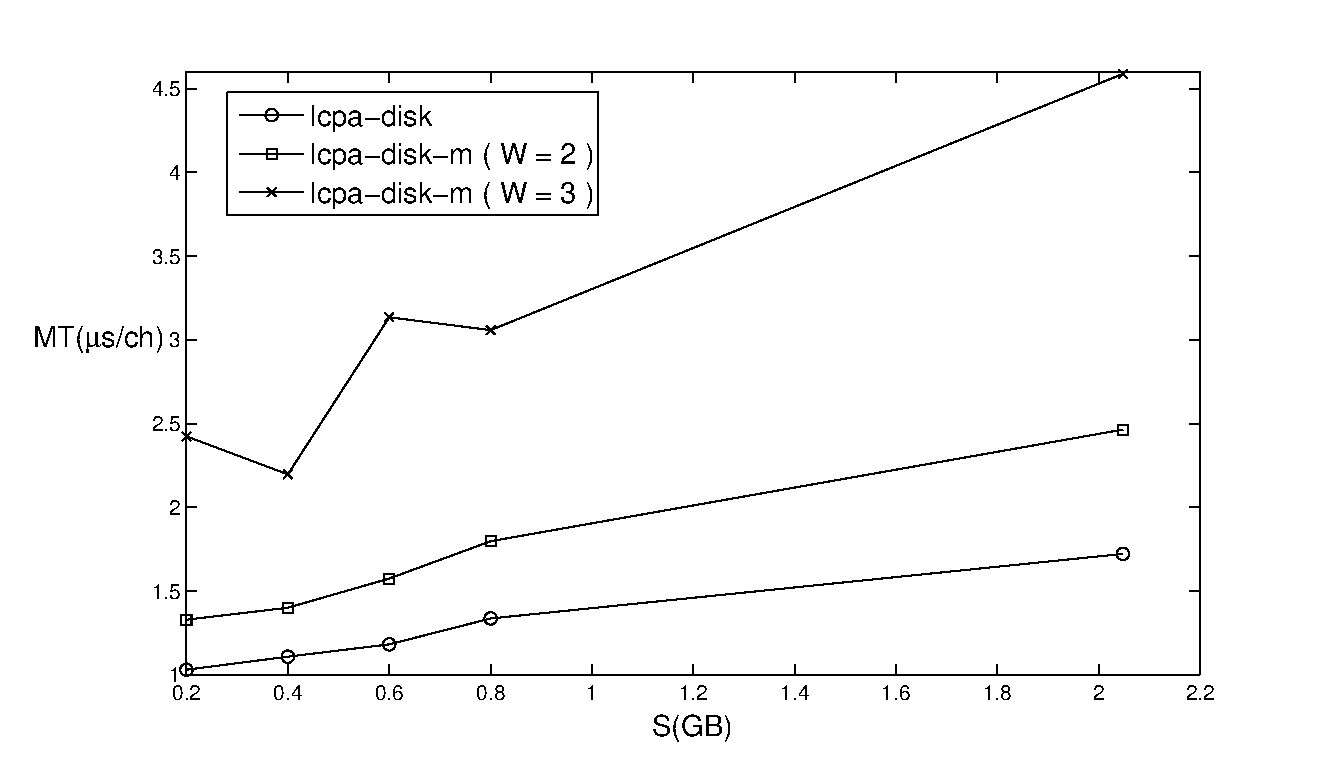
\includegraphics[scale=0.5]{disk_vs_diskm.eps}\\
  \caption{Performance comparison between lcpa-disk and lcpa-disk-m.}
  \label{fig:disk_vs_diskm}
\end{figure}


\subsection{lcpa-disk-m vs. lcpa-ds}

\begin{figure}[hbtp]
  \centering
  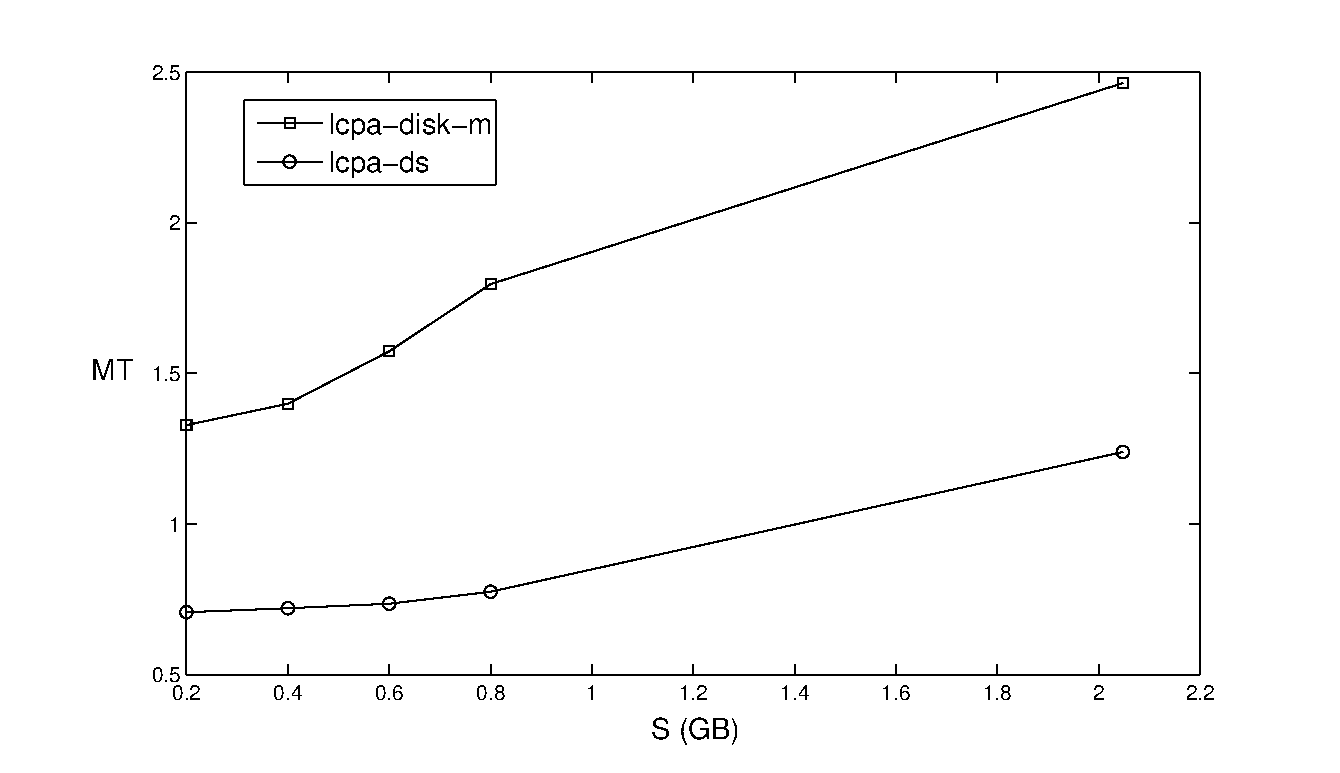
\includegraphics[scale=0.4]{diskm_vs_ds.eps}\\
  \caption{Performance comparison between lcpa-disk-m and lcpa-ds.}
  \label{fig:diskm_vs_ds}
\end{figure}

The distributed system for the program of lcpa-ds consists of 4 identical computing nodes, where each node adopts

the external algorithms lcpa-disk and lcpa-disk-m as well as the distributed algorithm lcpa-ds. The experimental platform for external programs is deployed on a computer equipped with two Intel Xeron E3-1220 CPUs, 4GB RAM and a 2TB disk,  running Ubuntu 14.04 operating system. The distributed one for lcpa-ds consists of 4 computing nodes. Each node adopts the platform for external programs and any two nodes are interconnected by a gigabit switch.


Each result in Table~\ref{tbl:exp:result} is a mean of two runs of the programs, where the running time and peak disk use are monitored by the shell command ``time" and ``stxxl::block\_manager", respectively.

performance analysis of STXXL

\subsection{lcpa-disk-m vs. lcpa-ds}


As can be seen, the running time of lcpa-disk-m is significantly faster than that of lcpa-disk in all cases, where the loop rounds of them are 7 and 13, respectively. We also observed that the processing time of each character per round varies from $1.99\ \mu s$ to $4.18\ \mu s$ as the size of corpora increases from 200 MiB to 2 GiB. This sub-linear phenomenon is partly due to the non-linear external memory sorts conducted by STXXL.

As reported in~\cite{Juha2014}, the disk space requirements for eSAIS and LCPscan are $65n$ and $21n$, respectively, while the peak disk use of the implementation for lcpa-disk-m rises up to $61n$ for processing the 2 GiB file. This indicates that {lcpa-disk-m} is more space demanding in comparison with the current best methods. However, the proposed method is easy to be implemented and strongly scalable for parallel and distributed models where the communication overhead on each node is balanced as $\mathcal{O}(\frac{n}{d})$.


\begin{table}
\caption{Loop rounds, mean running time in $\mu s/ch$ per round and peak disk use in bytes per character, where $K=8192$.}
\label{tbl:exp:result}
\centering
\begin{tabular}{|c|c|c|c|c|c|c|}
\hline
Size & \multicolumn{3}{c|}{lcpa-disk} & \multicolumn{3}{c|}{lcpa-disk-m} \\
\cline{2-7}
(MiB) & Round &  Time &  Disk & Round & Time &  Disk \\
\hline
200 & 13 & 1.71 & 30.94 & 7 & 1.99 & 47.36\\
\hline
400 & 13 & 1.70 & 31.50  & 7 & 2.01 & 47.36\\
\hline
600 & 13 & 1.79 & 31.58 & 7 & 2.27 & 47.36\\
\hline
800 & 13 & 1.86 & 31.52 & 7 & 2.65 & 47.38\\
\hline
1024 & 13 & 3.10 & 31.52 & 7 & 3.30 & 47.38\\
\hline
2048 & 13 & 3.16 & 46.04 & 7 & 4.18 & 60.48\\
\hline
\end{tabular}
\centering
\end{table}

\section{Conclusion}\label{sec:conclusion}

We present in this paper a practical $K$-order LCPA construction method that can be easily applied on both the internal memory and the external memory models. The program for lcpa-disk-m is less than 600 lines when using STXXL to implement the external sorts. We also show that the proposed method is straightforward to be extended for running on a typical distributed system of a cluster of $d$ computing nodes, where the time and space complexities are evenly divided onto each node as $\mathcal{O}(\frac{n}{d}\log K)$ and $\mathcal{O}(\frac{n}{d})$, respectively. The proposed algorithms are simple in design and universal for the RAM, disk and distributed models. Its implementations on all these models are not difficult and easily to be deployed.
A cluster of computers in a local area network are commonly available in practice, but there is currently lack of scalable LCPA construction algorithms for such a distributed model, in this sense, our algorithms provide a candidate solution to meet this demand. For further work, we now attempt to implement the distributed algorithm on a cluster of computers and speed up the computation of finger-prints by GPU.
\bibliographystyle{unsrt}
\bibliography{bibfile}

\end{document}


\begin{table}[b]
%\renewcommand{\arraystretch}{1.3}
\caption{Initial State and Arrivals}
\label{table:Initial State and Arrivals}
\centering
\begin{tabular}{|c|c|c|}
\hline
\multicolumn{3}{|c|}{Initial State($M=4,N=0$)}\\
\hline
\multicolumn{1}{|c}{Packet}&\multicolumn{1}{|c|}{Arrival Time Slot}&\multicolumn{1}{c|}{Searching Request}\\
\hline
$P_{1}$ & 0 & $R_{1}(m_{1},m_{2},m_{3},m_{4})$\\
\hline
$P_{2}$ & 1 & $R_{2}(m_{1},m_{3},m_{3},m_{2})$\\
\hline
$P_{3}$ & 2 & $R_{3}(m_{1},m_{4},m_{2},m_{3})$\\
\hline
$P_{4}$ & 3 & $R_{4}(m_{1},m_{4},m_{1},m_{2})$\\
\hline
$P_{5}$ & 4 & $R_{5}(m_{1},m_{1},m_{2},m_{3})$\\
\hline
$P_{6}$ & 5 & $R_{6}(m_{1},m_{2},m_{4},m_{1})$\\
\hline
$P_{7}$ & 6 & $R_{7}(m_{1},m_{3},m_{4},m_{4})$\\
\hline
$P_{8}$ & 7 & $R_{8}(m_{1},m_{2},m_{3},m_{1})$\\
\hline
\end{tabular}
\centering
\end{table}



\begin{figure}[!htbp]
\renewcommand{\figurename}{Fig.}
\centering
\subfigure[BT.]{\includegraphics[width=2.5in]{BT_D=1_H}
\label{fig:scheduling depth where $D=1$, BT}}
\subfigure[PT.]{\includegraphics[width=2.5in]{PT_D=1_H}
\label{fig:scheduling depth where $D=1$, PT}}
\subfigure[2-MPT.]{\includegraphics[width=2.5in]{MPT_D=1_H_correct}
\label{fig:scheduling depth where $D=1$, MPT}}
\subfigure[6-FST.]{\includegraphics[width=2.5in]{FST_D=1_H}
\label{fig:scheduling depth where $D=1$, FST}}
\caption{Performance comparison for the pipelined BT, PT, 2-MPT and 6-FST algorithms, with the memory accesses scheduled by FCFS, where $L=128$, $M=8$, $H\in \{8, 16, 32, 64, 128\}$ and $D=1$.}
\label{fig:scheduling depth where $D=1$}
\end{figure}


\begin{figure}[!htbp]
\renewcommand{\figurename}{Fig.}
\centering
\subfigure[BT.]{\includegraphics[width=2.5in]{BT_D_SA}
\label{fig:scheduling algorithms, BT}}
\subfigure[PT.]{\includegraphics[width=2.5in]{PT_D_SA}
\label{fig:scheduling algorithms, PT}}
\subfigure[2-MPT.]{\includegraphics[width=2.5in]{MPT_D_SA}
\label{fig:scheduling algorithms, MPT}}
\subfigure[6-FST.]{\includegraphics[width=2.5in]{FST_D_SA}
\label{fig:scheduling algorithms, FST}}
\caption{Performance comparison for the pipelined BT, PT, 2-MPT and 6-FST algorithms, with the memory accesses scheduled by FCFS, PIM and SLIP, where  $H=L=128$, $M=8$, $D\in \{1, 3\}$.}
\label{fig:scheduling algorithms}
\end{figure}
